% Bao cao tien do 28/10/2026. Bien dich bang pdfLaTeX mac dinh cua Overleaf.
% Mau Madrid, mau sac va bo cuc theo Reports/Presentation_23062026.tex.
% Dat companies_normalizer.png cung thu muc voi file nay neu muon chen anh o slide 4.
\documentclass{beamer}
\usepackage[utf8]{inputenc}
\usepackage[T5]{fontenc}
\usepackage[vietnamese]{babel}
\usepackage{graphicx}
\usepackage{booktabs}
\usepackage{tabularx}
\usepackage{array}

\usetheme{Madrid}
\usecolortheme{default}

\title[Tiến độ FollowUpAgent]{Báo cáo Tiến độ Dự án FollowUpAgent}
\subtitle{Review audio, chuẩn hóa transcript và cập nhật phân loại}
\author[]{Team UC-04}
\institute{}
\date{28 Tháng 10, 2026}

\newcommand{\code}[1]{{\ttfamily\detokenize{#1}}}

\begin{document}

% 1. Trang bia
\frame{\titlepage}

% 2. Muc luc thay cho timeline
\begin{frame}{Mục lục}
\begin{enumerate}
    \item Review và gán nhãn 50 audio đầu
    \item Companies text normalizer, audio im lặng và dữ liệu trùng
    \item Reason code, status group và summary
    \item Bảng hành động hiện tại của HR
    \item Lô 713 audio mới và các bước tiếp theo
\end{enumerate}
\end{frame}

% 3. Ground truth 50 audio
\begin{frame}{50 audio đầu: đã gán nhãn nhưng dữ liệu khó}
\begin{itemize}
    \item Nhóm đã nghe và gán nhãn ground truth cho \textbf{50 audio đầu}.
    \item Chất lượng phần lớn kém: nhiều cuộc gọi chỉ \textbf{5--10 giây}, lặp ``alo'', im lặng hoặc lỗi âm thanh.
    \item Một số cuộc gọi có tiếng nói nhưng nội dung \textbf{không liên quan tuyển dụng}.
    \item Lô này giúp tìm lỗi trong STT và classification; cần thận trọng khi dùng nó để kết luận chất lượng toàn hệ thống.
\end{itemize}
\end{frame}

% 4. Cho trong de chen anh
\begin{frame}{Thêm lớp companies text normalizer}
\begin{columns}[T,onlytextwidth]
    \begin{column}{0.48\textwidth}
        \begin{itemize}
            \item PhoWhisper thường ghi sai tên công ty và khu công nghiệp.
            \item Sau STT, normalizer sửa các cách nghe sai trước khi đưa transcript vào LLM.
            \item Ví dụ: ``lắc xê'' $\rightarrow$ \textbf{Luxshare}; ``vi xịt'' $\rightarrow$ \textbf{Vixech}.
            \item Prompt cũng nhận danh sách tên doanh nghiệp để viết summary đúng hơn.
        \end{itemize}
    \end{column}
    \begin{column}{0.48\textwidth}
        \centering
        \IfFileExists{companies_normalizer.png}{%
            \includegraphics[width=\linewidth,height=0.57\textheight,keepaspectratio]{companies_normalizer.png}%
        }{%
            \vspace*{0.18\textheight}
            {\large\textit{Chèn ảnh ví dụ transcript tại đây}}\par
            \vspace*{0.18\textheight}
        }
    \end{column}
\end{columns}
\end{frame}

% 5. Audio im lang va hallucination
\begin{frame}{Audio im lặng làm nhiễu transcript}
\begin{itemize}
    \item Khi audio hoàn toàn im lặng hoặc \textbf{10 giây đầu không có tiếng nói}, PhoWhisper vẫn có thể cố sinh chữ.
    \item Kết quả có thể lặp vô nghĩa: ``anh à, anh à, anh à...'' hoặc những câu không tồn tại trong audio.
    \item Transcript sai đi tiếp vào LLM và làm lệch reason code, status group, summary.
\end{itemize}
\begin{block}{Đã làm và phần còn thiếu}
Đã thêm \code{no_repeat_ngram_size=3} và \code{repetition_penalty=1.1} để giảm chữ lặp. Cần thêm bước phát hiện im lặng/không có lời nói trước STT; hai tham số trên chưa giải quyết được audio câm.
\end{block}
\end{frame}

% 6. Anh CSV minh hoa: cung call ID xuat hien nhieu lan
\begin{frame}{Ví dụ trong CSV: cùng call ID, cùng transcript}
\begin{center}
    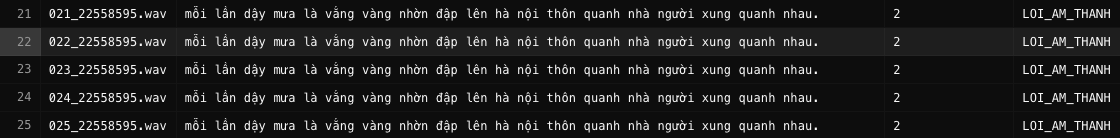
\includegraphics[width=\textwidth]{audio_repeated_transcript.png}
\end{center}
\vspace{0.25cm}
\begin{itemize}
    \item Năm dòng 021--025 đều mang call ID \code{22558595}; transcript giống hệt nhau và cùng được gán \code{LOI_AM_THANH}.
    \item Cần kiểm tra file audio gốc và bước tải file. Ảnh này chưa đủ để kết luận PhoWhisper đã sinh chữ từ im lặng.
\end{itemize}
\end{frame}

% 7. Reason code va status group
\begin{frame}{Sửa reason code và status group}
\begin{itemize}
    \item Qua quá trình nghe audio, nhóm tách các tình huống theo \textbf{hành động HR cần làm tiếp}: đóng hồ sơ, gọi lại, chăm sóc, nhắc lịch phỏng vấn, theo dõi sau khi chốt đi làm.
    \item Danh sách hiện tại có \textbf{5 status group và 12 reason code}. Các mã được định nghĩa cố định trong code.
    \item LLM chỉ chọn reason code hợp lệ. Hệ thống suy ra status group và \code{call_decision} từ mã đó, giúp lịch follow-up nhất quán.
    \item Ví dụ: ``đang bận, gọi lại sau'' khác với ``cần suy nghĩ thêm''; hai trường hợp cần lịch xử lý khác nhau.
\end{itemize}
\end{frame}

% 8. Summary
\begin{frame}{Summary cần đủ context cho HR}
\begin{itemize}
    \item Summary một câu thường bỏ sót việc ứng viên đã nói gì và hai bên chốt điều gì.
    \item Mục tiêu của nhóm là \textbf{2--3 câu}: bối cảnh cuộc gọi, thông tin/vướng mắc của ứng viên và kết quả hoặc mốc hẹn.
    \item HR cần đọc lại để nhớ đúng ứng viên và quyết định bước tiếp theo, thay vì phải suy đoán từ một nhãn ngắn.
\end{itemize}
\begin{block}{Điểm cần đồng bộ}
Prompt trong code hiện vẫn yêu cầu \textbf{3--5 câu}. Cần sửa về 2--3 câu và kiểm tra trên lô audio mới trước khi báo là đã áp dụng.
\end{block}
\end{frame}

% 9. Bang phan loai hien tai
\begin{frame}{Status group, reason code và hành động hiện tại}
\scriptsize
\renewcommand{\arraystretch}{1.12}
\begin{tabularx}{\textwidth}{@{}c p{1.65cm} X p{2.38cm}@{}}
\toprule
\textbf{Nhóm} & \textbf{Ý nghĩa} & \textbf{Reason code} & \textbf{Hành động / lịch}\\
\midrule
1 & Đóng hồ sơ & \code{TU_CHOI_LUON}\newline\code{KNM_DAP_MAY}\newline\code{SAI_SO_NHAM_SO} & \code{NO_CALL}; không lên lịch\\
\addlinespace[0.5ex]
2 & Cần gọi lại & \code{KHACH_BAN}\newline\code{CUOC_GOI_RONG}\newline\code{LOI_AM_THANH} & \code{CALL_BACK}; 2 giờ nếu khách bận, còn lại 15 phút\\
\addlinespace[0.5ex]
3 & Cần chăm sóc & \code{SUY_NGHI_THEM}\newline\code{CHUA_CHOT_NGAY}\newline\code{CHO_GIAY_TO}\newline\code{HEN_XA} & \code{FOLLOW_UP}; sau 3 ngày\\
\addlinespace[0.5ex]
4 & Đã hẹn phỏng vấn & \code{HEN_PHONG_VAN} & \code{SCHEDULED}; nhắc trước hẹn 1 ngày\\
\addlinespace[0.5ex]
5 & Chốt đi làm & \code{DI_LAM} & \code{SUCCESS}; theo dõi sau 2 ngày\\
\bottomrule
\end{tabularx}
\end{frame}

% 10. Batch moi
\begin{frame}{Lô 713 audio mới}
\begin{itemize}
    \item Nhóm vừa nhận \textbf{713 audio ghi âm mới}, chất lượng nghe tốt hơn lô 50 audio đầu.
    \item Đã chuẩn bị đường tải từ API \code{/recordings} và script auto-label có thể chạy tiếp khi bị ngắt.
    \item Khối lượng gán nhãn lớn hơn \textbf{14 lần} lô đầu; cần kiểm tra đủ WAV, nghe mẫu và theo dõi lỗi STT/LLM trong lúc chạy.
    \item Nhãn AI trong CSV là gợi ý ban đầu. Ground truth vẫn cần người nghe và xác nhận.
\end{itemize}
\end{frame}

% 11. Next steps
\begin{frame}{Các bước tiếp theo}
\begin{enumerate}
    \item Đối chiếu 713 ID với số WAV tải thành công; nghe mẫu trước khi chạy full batch.
    \item Thêm kiểm tra audio im lặng/không có lời nói, nhất là đoạn đầu cuộc gọi.
    \item Đồng bộ prompt summary về mục tiêu 2--3 câu rồi kiểm tra trên audio thật.
    \item Chạy auto-label có resume; người nghe điền nhãn ground truth và ghi lại các trường hợp khó.
    \item So nhãn AI với nhãn người, rà các reason code dễ nhầm và điều chỉnh lịch follow-up nếu cần.
\end{enumerate}
\end{frame}

\end{document}
